\chapter{Desarrollo del Framework}

En este capitulo, trataremos los asuntos concernientes a la construcción de las
funciones del framework, sobre las que recaen la automatización de los casos de
prueba, y la expansibilidad que pueda darse a todo el proyecto.

Si bien en el anterior capitulo el tema fundamental era el análisis y
exploración que se realizo sobre el software, el objeto central de este
capitulo es el framework mismo.

\section{Casos de prueba}
A partir del análisis realizado en el anterior capitulo, se termino formulando
múltiples casos de prueba, estos se encuentran descritos en el \textbf{apéndice
\ref{appendix}} categorizados e individualizados según el área y suba rea al que
pertenecen.

\section{Código fuente}
Todo el código fuente del framework se encuentra versionado y disponible desde
github, en la siguiente dirección:
\\
\\
\centerline{\textbf{https://github.com/ccaballero/salesforce\_automation}}

\section{Estructura del Framework}
El framework desarrollado basa su estructura y comportamiento en las
recomendaciones de la biblioteca utilizada (\emph{webdriver.io}), esta puede
verse en la figura \ref{estructura}.

\begin{figure}
\centering
\begin{tikzpicture}[
    grow via three points={one child at (0.5,-0.7) and
    two children at (0.5,-0.7) and (0.5,-1.4)},
    edge from parent path={(\tikzparentnode.south) |- (\tikzchildnode.west)}]
    \node {salesforce\_automation}
        child { node {Errors}}
        child { node {PageObjects}
            child { node {New}
                child { node {ListView.po.js}}
                child { node {PriceBook.po.js}}
                child { node {Product.po.js}}
            }
            child [missing] {}
            child [missing] {}
            child [missing] {}
            child { node {Card.po.js}}
            child { node {Confirmation.po.js}}
            child { node {Launcher.po.js}}
            child { node {List.po.js}}
            child { node {Login.po.js}}
            child { node {Message.po.js}}
            child { node {Modal.po.js}}
            child { node {Profile.po.js}}
            child { node {Row.po.js}}
            child { node {Setup.po.js}}
            child { node {View.po.js}}
        }
        child [missing] {}
        child [missing] {}
        child [missing] {}
        child [missing] {}
        child [missing] {}
        child [missing] {}
        child [missing] {}
        child [missing] {}
        child [missing] {}
        child [missing] {}
        child [missing] {}
        child [missing] {}
        child [missing] {}
        child [missing] {}
        child [missing] {}
        child { node {Specs}
            child { node {001.F001.js}}
            child { node {002.F002.js}}
            child { node {003.A001.js}}
            child { node {\ldots.js}}
        }
        child [missing] {}
        child [missing] {}
        child [missing] {}
        child [missing] {}
        child { node {Utils}
            child { node {Common.js}}
        }
        child [missing] {}
        child { node {config.js}}
        child { node {package.json}}
        child { node {wdio.conf.js}};
\end{tikzpicture}
\caption{Estructura de archivos del Framework.}
\label{estructura}
\end{figure}

Puede observarse en esta figura, que se creó la carpeta \textbf{PageObjects}
para albergar todas las clases que representan elementos de las paginas que
componen el framework, además de una carpeta \textbf{Specs} que alberga los
casos de prueba automatizados, adicionalmente existe la carpeta \textbf{Utils}
donde se ubicaron Clases adicionales utilitarias.

Adicionalmente a estas carpetas también se encuentran los ficheros relacionados
con la biblioteca webdriver.io, utilizados como se detallan a continuación:

\begin{description}
\item [config.dist.js] Archivo de configuración del framework, sin
    credenciales para ser versionado con el sistema de control de cambios.
\item [config.js] Archivo de configuración del framework, donde están
    parametrizados todas las variables y credenciales necesarias durante la
    ejecución.
\item [docker-compose.yml] Archivo de orquestación de imágenes utilizados para
    la ejecución de los casos de prueba sobre imágenes de \emph{Docker}.
\item [package.json] Archivo de configuración de node.js, que incluye los
    diferentes tipos de ejecución disponible, las bibliotecas utilizadas, entre
    otros detalles menores acerca del proyecto.
\item [wdio.browserstack.conf.js] Archivo de configuración utilizado por la
    biblioteca \emph{webdriver.io} para la ejecución de las pruebas sobre el
    servicio \emph{BrowserStack}.
\item [wdio.conf.js] Archivo de configuración de \emph{webdriver.io}, este
    contiene las conjuntos de pruebas disponibles, entre otras variables
    utilizadas por el entorno de prueba.
\item [wdio.docker.conf.js] Archivo de configuración utilizado por la
    biblioteca \emph{webdriver.io} para la ejecución de las pruebas sobre el
    servidor \emph{Docker}.
\item [wdio.standalone.conf.js] Archivo de configuración utilizado por la
    biblioteca \emph{webdriver.io} para la ejecución de las pruebas sobre el
    mismo ordenador en modo solitario.
\end{description}

\section{Suites Disponibles}
El proyecto ha sido configurado de forma que puedan ejecutarse diferentes
conjuntos de casos de prueba, estos se detallan en el cuadro \ref{suites}.

\begin{table}
\centering
\begin{tabular}{|l|p{12.0cm}|}
\hline
\footnotesize{\textbf{Suite}} & \footnotesize{\textbf{Descripción}} \\
\hline
\footnotesize{\emph{init}} & \footnotesize{Ejecución de una prueba rápida de
disponibilidad de la URL principal de \emph{Salesforce} a evaluar.} \\
\footnotesize{\emph{login}} & \footnotesize{Ejecución de una prueba rápida de
acceso al sistema, útil para verificación de credenciales.} \\
\footnotesize{\emph{products}} & \footnotesize{Ejecución de todos los casos de
prueba relacionados con el modulo de gestión  de productos.} \\
\footnotesize{\emph{pricebooks}} & \footnotesize{Ejecución de todos los casos de
prueba relacionados con el modulo de gestión de listas de precios.} \\
\footnotesize{\emph{listviews}} & \footnotesize{Ejecución de todos los casos de
prueba relacionados con el modulo de gestión de vistas de listas.} \\
\footnotesize{\emph{functional}} & \footnotesize{Ejecución de todos los casos de
prueba relacionados con pruebas funcionales en todos los módulos.} \\
\footnotesize{\emph{acceptance}} & \footnotesize{Ejecución de todos los casos de
prueba relacionados con pruebas de aceptación en todos los módulos.} \\
\footnotesize{\emph{negative}} & \footnotesize{Ejecución de todos los casos de
prueba relacionados con pruebas negativas en todos los módulos.} \\
\footnotesize{\emph{domain}} & \footnotesize{Ejecución de todos los casos de
prueba relacionados con pruebas de dominio en todos los módulos.} \\
\hline
\end{tabular}
\caption{Suites en el framework para las diferentes etapas de evaluación.}
\label{suites}
\end{table}

\section{\emph{Page Objects Model}}
Los \emph{Page Objects} representan el corazón del proyecto de automatización,
estos representan las diferentes paginas a ser testeadas y algunos de sus
componentes que posean cierto grado de complejidad.

Si bien los \emph{Page Objects} son clases instanciables en \emph{javascript},
la mayor parte son utilizados de manera estática y con un relacionamiento
entre estos que es dinámico y sustancialmente inexistente, aun así puede
utilizarse un diagrama de clases convencional para comprender las relaciones
entre estos como se presenta en la figura \ref{pom}.

\begin{figure}
\centering
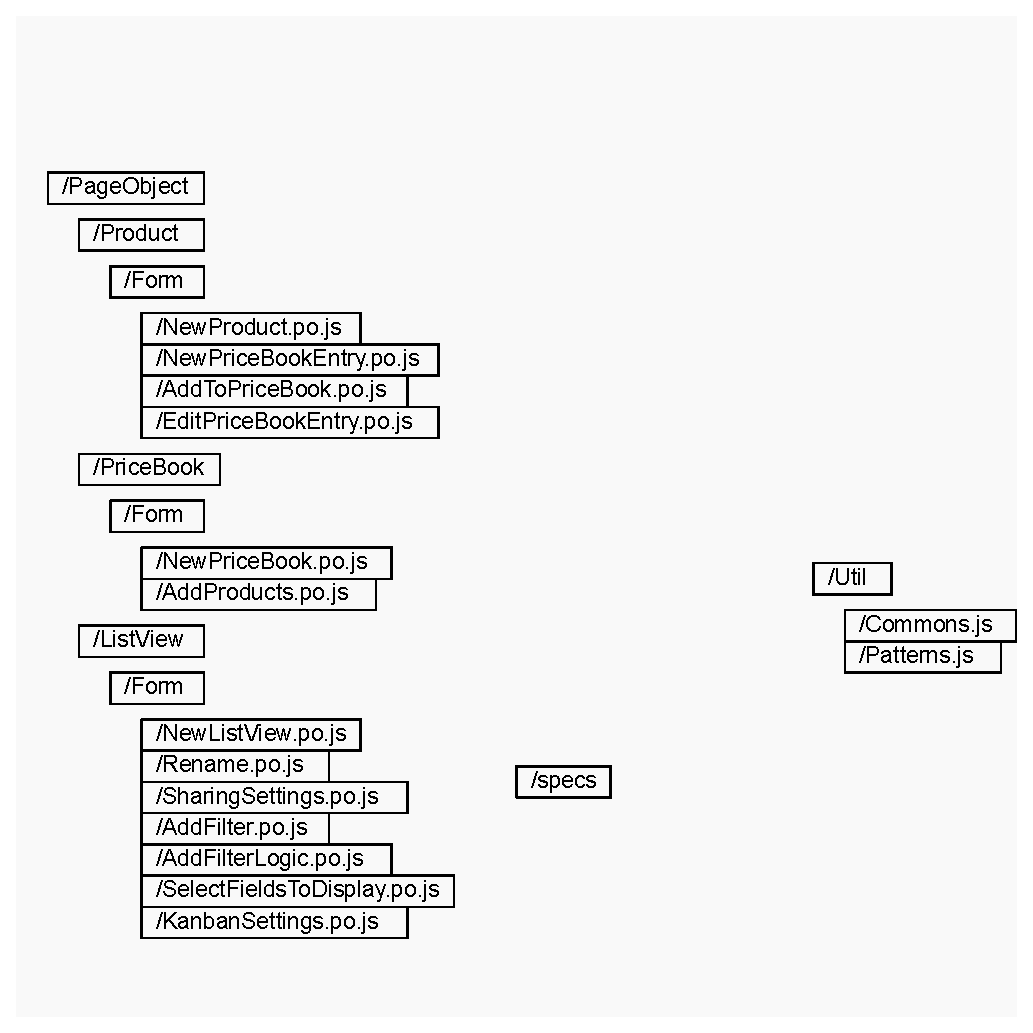
\includegraphics[width=1.0\textwidth]{graphics/diagram01.eps}
\caption{Diagrama de clases sobre las relaciones entre \emph{Page Objects}.}
\label{pom}
\end{figure}

\section{\emph{Specs}}
Los \emph{Specs} representan las rutinas de automatización propiamente dichas,
en estas se encuentran la implementación de los casos de prueba; para el
proyecto se ha intentando hacer de estos lo mas expresivos posibles de forma
que su legibilidad sea la mayor, en la figura \ref{lltc} se muestra el caso de
prueba A001, y en la figura \ref{spec} se ve reflejado el código de ejecución
automatizado.

\begin{figure}
\centering
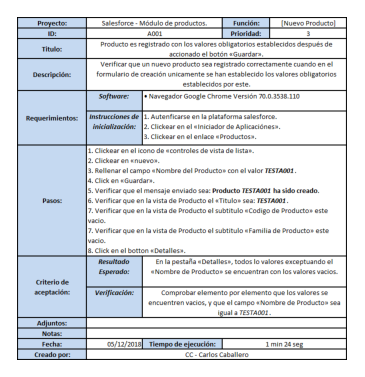
\includegraphics[width=1.0\textwidth]{graphics/lltc.eps}
\caption{Especificación del Caso de Prueba.}
\label{lltc}
\end{figure}

\begin{figure}
\begin{verbatim}
it('A001 - Producto es registrado con los valores obligatorios '+
   'establecidos después de accionado el botón «Guardar»',()=>{
    let modal_new=Launcher.app('Products').new()
      , message=modal_new
            .fill({
                name:name
            })
            .save();

    expect(message.result()).to.equal('success');
    expect(message.text()).to.equal('Product "'+name+'" was created.');

    message.close();

    let view=new View();

    expect(view.title()).to.equal(name);
    expect(view.subtitle('Product Code')).to.equal('');
    expect(view.subtitle('Product Family')).to.equal('');

    view.details();

    expect(view.data('Product Name')).to.equal(name);
    expect(view.checked('Active')).to.equal(false);
    expect(view.data('Product Code')).to.equal('');
    expect(view.data('Product Family')).to.equal('');
    expect(view.checked('Quantity Scheduling Enabled')).to.equal(false);
    expect(view.checked('Revenue Scheduling Enabled')).to.equal(false);
    expect(view.data('Product Description')).to.equal('');

    view.options()
        .delete()
        .confirm();
});
\end{verbatim}
\caption{Automatización del Caso de Prueba A001.}
\label{spec}
\end{figure}

Este \emph{spec} que cubre la automatización del caso de prueba A001, utiliza
cinco \emph{Page Objects}, dos utilizadas para la ejecución de las
precondiciones del test, y tres para realizar la secuencia de pasos, como puede
verse en el diagrama de secuencia de la figura \ref{sequence}.

\begin{figure}
\centering
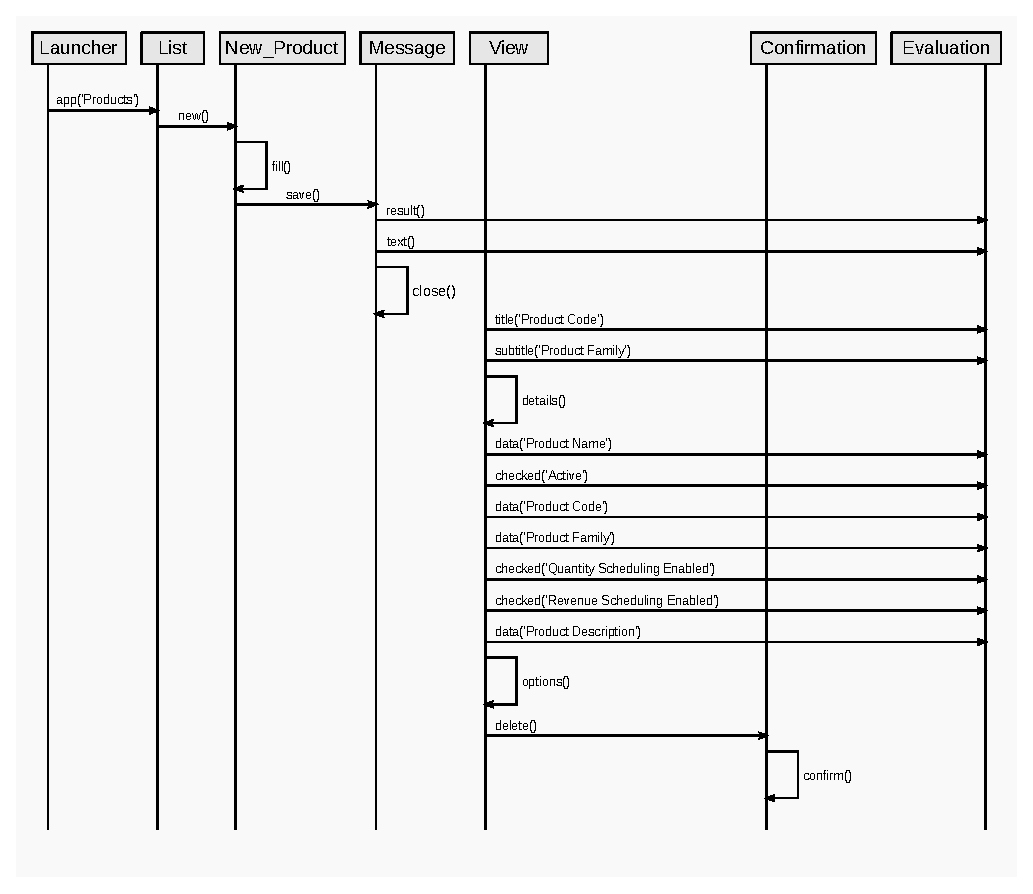
\includegraphics[width=1.0\textwidth]{graphics/diagram02.eps}
\caption{Diagrama de secuencia para el \emph{spec} del caso de prueba A001.}
\label{sequence}
\end{figure}

\section{Ejecución de las pruebas}
En la figura \ref{tc-tests}, se puede ver la distribución de los casos de prueba
según el tipo de evaluación realizado, puede apreciarse que las pruebas
funcionales ocupan mas de la mitad de la totalidad de casos de prueba en el
proyecto, mientras que los casos de prueba negativos, y de aceptación, están más
próximos al 10\%.

En la figura \ref{tc-type}, se puede ver la distribución de los casos de prueba
según el tipo de acción que se realiza en el sistema, es decir, si son casos
que afectan la interfaz de usuario, si mas bien son funciones de validación, o
si realizan alguna petición al servidor, sea esta de lectura o escritura.

\begin{figure}[H]
\centering
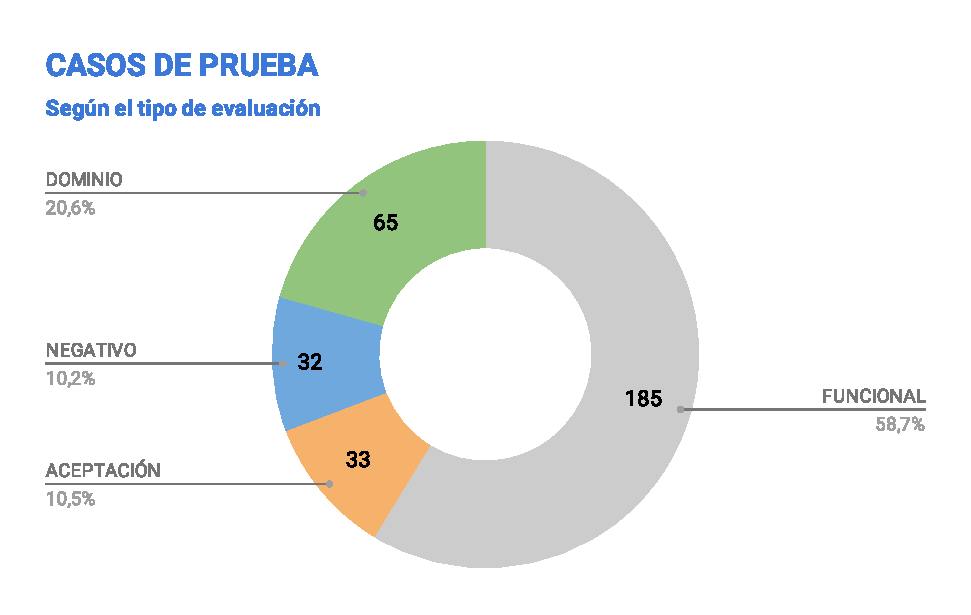
\includegraphics[width=1.0\textwidth]{graphics/tc-tests.eps}
\caption{Casos de Prueba según el tipo de evaluación realizada.}
\label{tc-tests}
\end{figure}

\begin{figure}[H]
\centering
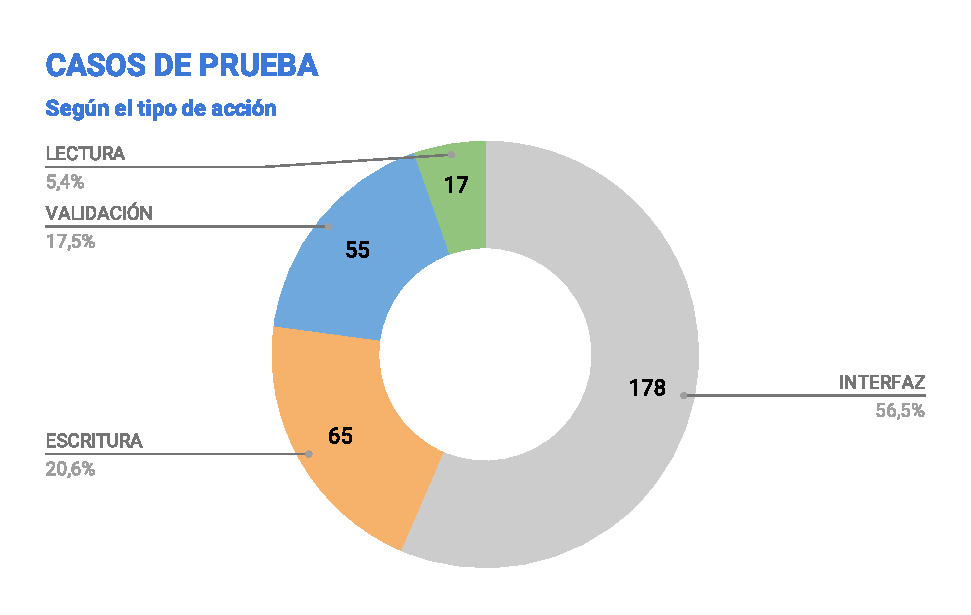
\includegraphics[width=1.0\textwidth]{graphics/tc-type.eps}
\caption{Casos de Prueba según el tipo de acción a evaluar.}
\label{tc-type}
\end{figure}

Puede apreciarse igualmente que la mayor parte de los casos de prueba están
orientados a evaluar el comportamiento de la interfaz de usuario, mientras que
en un 25\% aproximadamente se evalúan funcionalidades que se comunican con el
servidor.

En las figuras \ref{results-tests} y \ref{results-type}, se condensan los
resultados obtenidos de la ejecución de los casos de prueba, en los cuales
únicamente fallaron 2 casos de prueba, ambos relacionados a un mismo formulario,
como puede verse en el reporte de error adjunto, y debido al fallo de estos
también se bloquearon dos casos de prueba.

\begin{figure}[H]
\centering
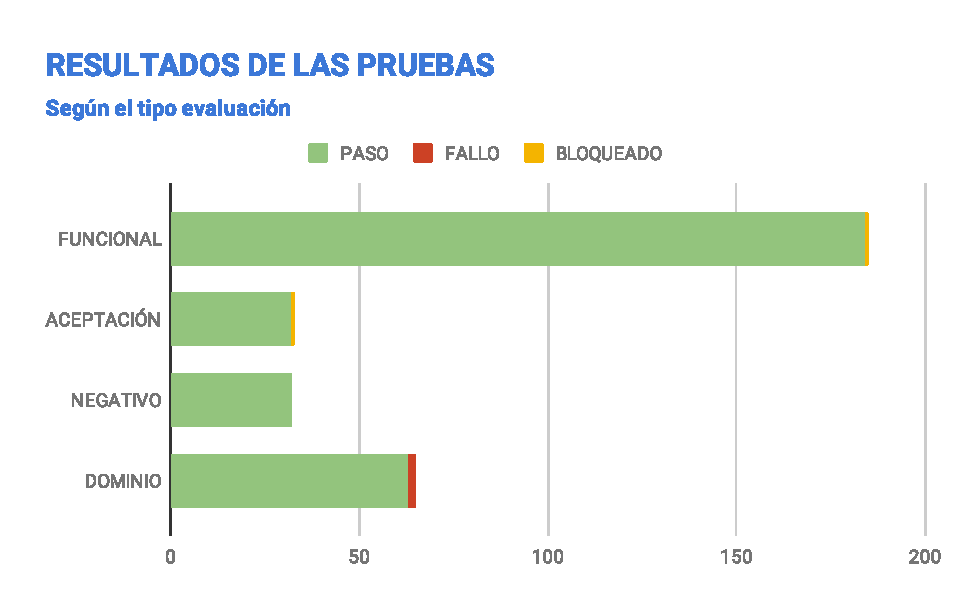
\includegraphics[width=1.0\textwidth]{graphics/results-tests.eps}
\caption{Resultados de las pruebas clasificadas por tipo de evaluación.}
\label{results-tests}
\end{figure}

\begin{figure}[H]
\centering
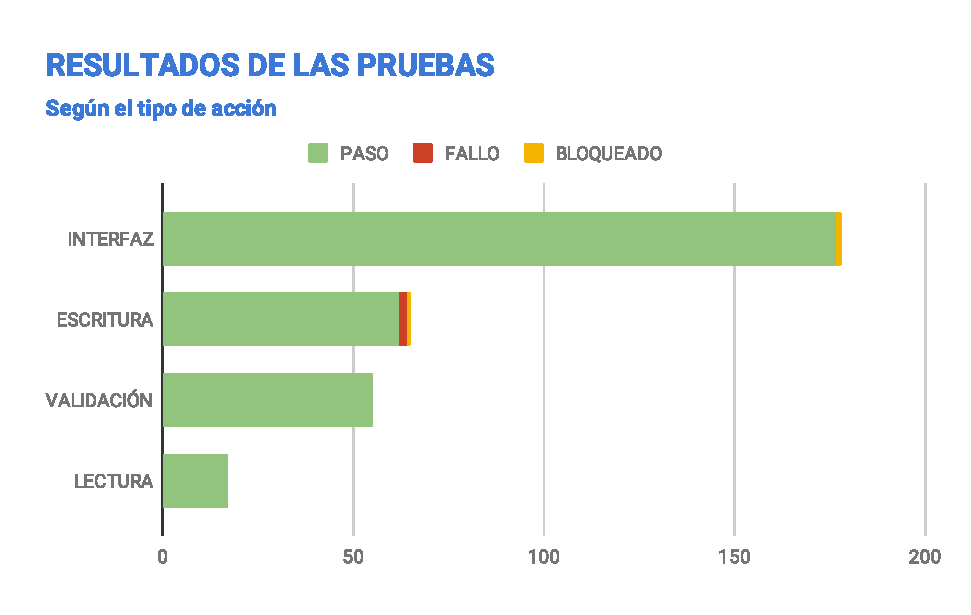
\includegraphics[width=1.0\textwidth]{graphics/results-type.eps}
\caption{Resultados de las pruebas clasificadas por tipo de acción a evaluar.}
\label{results-type}
\end{figure}

Presentados los resultados de la ejecución de las pruebas, vemos que de los 315
casos de pruebas únicamente existen 2 bloqueados, y dos fallidos. Por ende se
tiene 98.74\% de casos de prueba exitosos, lo que lleva a concluir que los
atributos de calidad esperados del sistema están cubiertos por completo.

